\section{Vectores}

En física e ingeniería, muchas cantidades como la temperatura o la masa pueden describirse completamente con un solo número real; a estas cantidades se les llama \textbf{escalares}. Sin embargo, cantidades como la fuerza, la velocidad o el desplazamiento requieren de una magnitud (tamaño) y una dirección espacial para estar completamente definidas. A estas cantidades las llamamos \textbf{vectores}.
Geométricamente, un vector se representa como un segmento de recta dirigido (una flecha). El punto donde comienza la flecha se llama \textit{punto inicial} (u origen) y la punta de la flecha es el \textit{punto final}.

\subsection{Vectores en $\mathbb{R}^n$}

Aunque es fácil visualizar vectores en 2 o 3 dimensiones, en matemáticas y ciencias de la computación es común trabajar con sistemas que tienen múltiples variables o grados de libertad. Para esto, extendemos la definición geométrica a una definición algebraica de $n$ dimensiones (o $n$ entradas).

\begin{mydefinition}{Vector en $\mathbb{R}^n$}
Un vector $\vec{v}$ en un espacio $n$-dimensional ($\mathbb{R}^n$) se define como una lista ordenada de $n$ números reales, llamados las \textbf{componentes} o \textbf{entradas} del vector. Se denota como:
$$ \vec{v} = (v_1, v_2, v_3, \dots, v_n) $$
Donde cada $v_i \in \mathbb{R}$ representa la magnitud del vector en la dirección del $i$-ésimo eje coordenado.
\end{mydefinition}

\subsection{Vectores libres e invarianza bajo traslación}

En el estudio del álgebra vectorial, es crucial entender que un vector está completamente definido por solo dos atributos: su \textbf{magnitud} y su \textbf{dirección}. El punto específico del espacio donde el vector comienza no altera su identidad matemática.

Esta propiedad significa que podemos tomar un vector y trasladarlo libremente a cualquier otra parte del plano o del espacio, siempre y cuando no sea girado ni estirado. 

\begin{mydefinition}{Vectores libres y equivalentes}
Dos o más vectores son \textbf{equivalentes} si tienen exactamente la misma magnitud y la misma dirección. En matemáticas y en muchas aplicaciones de ingeniería, los vectores se consideran \textbf{vectores libres}, lo que significa que un vector y cualquiera de sus traslaciones en el espacio representan exactamente al mismo objeto matemático.
\end{mydefinition}

\subsubsection{Vectores de posición vs. Vectores libres}
Aunque podemos dibujar un vector comenzando en cualquier lugar, para facilitar los cálculos algebraicos es práctica común trasladarlo para que su punto inicial coincida con el origen del sistema de coordenadas $(0,0)$ o $(0,0,0)$. Cuando un vector libre comienza en el origen, se le llama \textbf{vector de posición}.

\begin{center}
\shorthandoff{>}
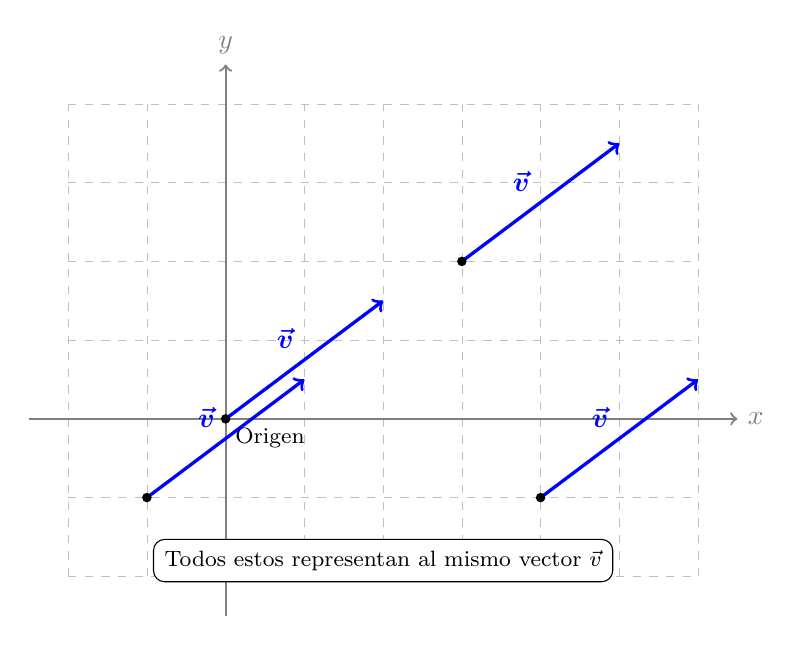
\begin{tikzpicture}[scale=1]
    \draw[lightgray, very thin, dashed] (-2,-2) grid (6,4);
    
    \draw[->, gray, thick] (-2.5,0) -- (6.5,0) node[right] {$x$};
    \draw[->, gray, thick] (0,-2.5) -- (0,4.5) node[above] {$y$};
    
    \draw[->, very thick, blue] (0,0) -- (2,1.5) node[midway, above left, font=\boldmath] {$\vec{v}$};
    \filldraw[black] (0,0) circle (1.5pt) node[below right] {\footnotesize Origen};
    
    \draw[->, very thick, blue] (3,2) -- (5,3.5) node[midway, above left, font=\boldmath] {$\vec{v}$};
    \draw[->, very thick, blue] (-1,-1) -- (1,0.5) node[midway, above left, font=\boldmath] {$\vec{v}$};
    \draw[->, very thick, blue] (4,-1) -- (6,0.5) node[midway, above left, font=\boldmath] {$\vec{v}$};
    
    \filldraw[black] (3,2) circle (1.5pt);
    \filldraw[black] (-1,-1) circle (1.5pt);
    \filldraw[black] (4,-1) circle (1.5pt);
    
    \node[fill=white, draw=black, rounded corners, inner sep=4pt] at (2, -1.8) 
    {\footnotesize Todos estos representan al mismo vector $\vec{v}$};
\end{tikzpicture}
\end{center}

\subsection{Multiplicación por un escalar}

La multiplicación escalar es la operación de multiplicar un vector por un número real (escalar) $\kappa$. Geométricamente, esto altera la longitud (magnitud) del vector. 
\begin{itemize}
    \item Si $\kappa > 1$, el vector se \textit{estira} o dilata.
    \item Si $0 < \kappa < 1$, el vector se \textit{contrae}.
    \item Si $\kappa < 0$, el vector cambia a la \textit{dirección opuesta} (invierte su sentido).
\end{itemize}
Sin embargo, el vector resultante siempre es paralelo al vector original (se mantiene sobre la misma línea de acción).

\begin{center}
\shorthandoff{>}
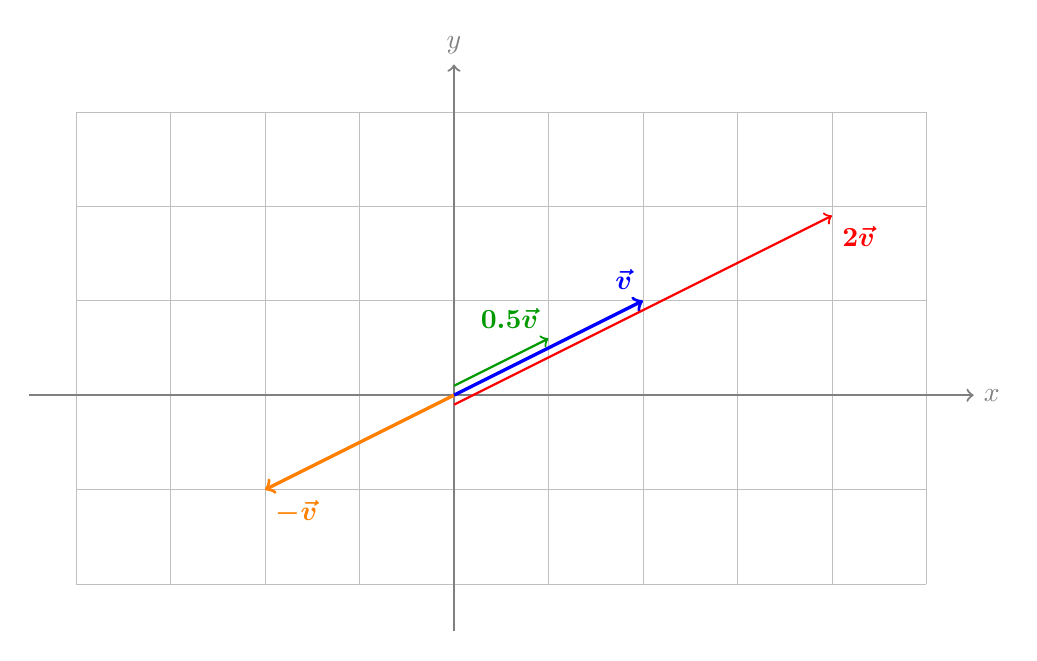
\begin{tikzpicture}[scale=1.2]
    % Cuadrícula y ejes de fondo para referencia
    \draw[lightgray, very thin] (-4,-2) grid (5,3);
    \draw[->, thick, gray] (-4.5,0) -- (5.5,0) node[right] {$x$};
    \draw[->, thick, gray] (0,-2.5) -- (0,3.5) node[above] {$y$};

    % Vector original v
    \draw[->, very thick, blue] (0,0) -- (2,1) node[above left, font=\boldmath] {$\vec{v}$};
    
    % Escalar 2: Estiramiento (dibujado ligeramente desplazado para que se vea)
    \draw[->, thick, red, yshift=-0.1cm] (0,0) -- (4,2) node[below right, font=\boldmath] {$2\vec{v}$};
    
    % Escalar 0.5: Contracción (dibujado ligeramente desplazado hacia arriba)
    \draw[->, thick, green!60!black, yshift=0.1cm] (0,0) -- (1,0.5) node[above left, font=\boldmath] {$0.5\vec{v}$};
    
    % Escalar -1: Inversión de sentido
    \draw[->, very thick, orange] (0,0) -- (-2,-1) node[below right, font=\boldmath] {$-\vec{v}$};
    
\end{tikzpicture}
\end{center}

\subsection{Suma de vectores en $\mathbb{R}^2$}

Para sumar dos vectores $\vec{u}$ y $\vec{v}$ geométricamente, se utiliza la \textbf{Regla del Paralelogramo} o el método de "punta a cola". Si colocamos el punto inicial de $\vec{v}$ en el punto final de $\vec{u}$, el vector suma $\vec{u} + \vec{v}$ es la flecha que va desde el origen de $\vec{u}$ hasta la punta de $\vec{v}$.

\begin{center}
\shorthandoff{>}
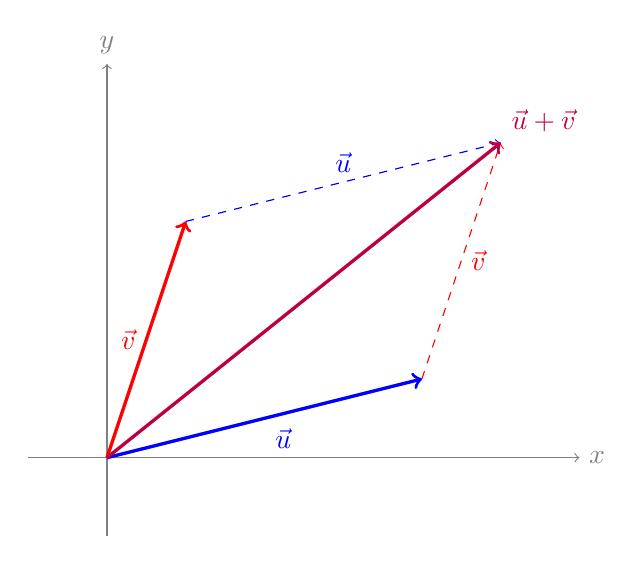
\begin{tikzpicture}[scale=1]
    % Ejes
    \draw[->, gray] (-1,0) -- (6,0) node[right] {$x$};
    \draw[->, gray] (0,-1) -- (0,5) node[above] {$y$};

    % Vectores u y v
    \draw[->, very thick, blue] (0,0) -- (4,1) node[midway, below right] {$\vec{u}$};
    \draw[->, very thick, red] (0,0) -- (1,3) node[midway, left] {$\vec{v}$};

    % Proyecciones para el paralelogramo
    \draw[->, dashed, red] (4,1) -- (5,4) node[midway, right] {$\vec{v}$};
    \draw[->, dashed, blue] (1,3) -- (5,4) node[midway, above] {$\vec{u}$};

    % Vector Suma
    \draw[->, very thick, purple] (0,0) -- (5,4) node[above right] {$\vec{u} + \vec{v}$};
\end{tikzpicture}
\end{center}

\subsection{Sustracción de vectores}

La resta de dos vectores se define algebraicamente a partir de la suma y la multiplicación escalar. Restar $\vec{v}$ de $\vec{u}$ es lo mismo que sumarle a $\vec{u}$ el negativo de $\vec{v}$:

\[ \vec{u} - \vec{v} = \vec{u} + (-\vec{v}) \] 

Geométricamente, si graficamos $\vec{u}$ y $\vec{v}$ desde el mismo origen, el vector $\vec{u} - \vec{v}$ es el vector que va desde la punta de $\vec{v}$  hasta la punta de $\vec{u}$.

\begin{center}
\shorthandoff{>}
\begin{tikzpicture}[scale=1]
    \draw[->, gray] (-2,0) -- (5,0) node[right] {$x$};
    \draw[->, gray] (0,-3) -- (0,4) node[above] {$y$};

    \draw[->, very thick, blue] (0,0) -- (4,2) node[above right] {$\vec{u}$};
    \draw[->, very thick, red] (0,0) -- (1,3) node[above left] {$\vec{v}$};

    \draw[->, dashed, orange] (0,0) -- (-1,-3) node[below left] {$-\vec{v}$};
    
    \draw[->, dashed, blue] (-1,-3) -- (3,-1);
    \draw[->, dashed, orange] (4,2) -- (3,-1);
    
    \draw[->, very thick, purple] (0,0) -- (3,-1) node[below right] {$\vec{u} - \vec{v}$};

    \draw[->, very thick, purple, dashed] (1,3) -- (4,2) node[midway, above right] {$\vec{u} - \vec{v}$};
\end{tikzpicture}
\end{center}

\subsection{Generalización de operaciones en $\mathbb{R}^n$}

Las operaciones que visualizamos en $\mathbb{R}^2$ se definen algebraicamente componente a componente para cualquier vector en $\mathbb{R}^n$.

Sean $\vec{u} = (u_1, u_2, \dots, u_n)$ y $\vec{v} = (v_1, v_2, \dots, v_n)$ dos vectores en $\mathbb{R}^n$, y sea $\kappa \in \mathbb{R}$ un escalar. Entonces, las operaciones fundamentales se definen como:

\begin{mydefinition}{Operaciones vectoriales en $\mathbb{R}^n$}
\textbf{1. Suma vectorial:}
\[\vec{u} + \vec{v} = (u_1 + v_1, u_2 + v_2, \dots, u_n + v_n)\]

\textbf{2. Multiplicación por un escalar:}
\[\kappa\vec{u} = (\kappa u_1, \kappa u_2, \dots, \kappa u_n)\]

\textbf{3. Resta vectorial:}
\[\vec{u} - \vec{v} = (u_1 - v_1, u_2 - v_2, \dots, u_n - v_n)\]
\end{mydefinition}

\subsection{Propiedades fundamentales de los vectores}

Las operaciones que definimos anteriormente siguen axiomas específicos. Estas propiedades son la base para manipular ecuaciones vectoriales en el cálculo multivariable y el álgebra lineal.

Sean $\vec{u}$, $\vec{v}$ y $\vec{w}$ vectores en $\mathbb{R}^n$, y sean $\kappa$ y $\lambda$ escalares (números reales). Se cumplen las siguientes propiedades:

\begin{mytheorem}{Propiedades del Álgebra Vectorial}
\begin{enumerate}
    \item \textbf{Conmutatividad de la suma:} $\vec{u} + \vec{v} = \vec{v} + \vec{u}$
    \item \textbf{Asociatividad de la suma:} $(\vec{u} + \vec{v}) + \vec{w} = \vec{u} + (\vec{v} + \vec{w})$
    \item \textbf{Elemento neutro aditivo:} Existe un vector cero $\vec{0} = (0,0,\dots,0)$ tal que $\vec{u} + \vec{0} = \vec{u}$
    \item \textbf{Inverso aditivo:} Para cada $\vec{u}$, existe un vector $-\vec{u}$ tal que $\vec{u} + (-\vec{u}) = \vec{0}$
    \item \textbf{Distributividad del escalar sobre suma vectorial:} $\kappa(\vec{u} + \vec{v}) = \kappa\vec{u} + \kappa\vec{v}$
    \item \textbf{Distributividad del escalar sobre suma escalar:} $(\kappa + \lambda)\vec{u} = \kappa\vec{u} + \lambda\vec{u}$
    \item \textbf{Asociatividad de la multiplicación escalar:} $\kappa(\lambda\vec{u}) = (\kappa\lambda)\vec{u}$
    \item \textbf{Elemento neutro multiplicativo:} $1\vec{u} = \vec{u}$
\end{enumerate}
\end{mytheorem}

\subsection{Magnitud de un vector}

La \textbf{magnitud}, \textbf{longitud} o \textbf{norma} de un vector es una medida escalar que representa el ``tamaño'' del vector. Físicamente, si el vector representa un desplazamiento, su magnitud es la distancia rectilínea entre su punto inicial y su punto final.

\subsubsection{La magnitud en $\mathbb{R}^2$ y el teorema de pitágoras}

En el plano bidimensional ($\mathbb{R}^2$), cualquier vector $\vec{v} = (v_1, v_2)$ puede visualizarse como la hipotenusa de un triángulo rectángulo, donde los catetos están formados por las proyecciones del vector sobre los ejes $x$ e $y$.

Por lo tanto, la magnitud del vector, denotada como $\|\vec{v}\|$, se calcula aplicando directamente el \textbf{teorema de pitágoras}:

\begin{center}
\shorthandoff{>}
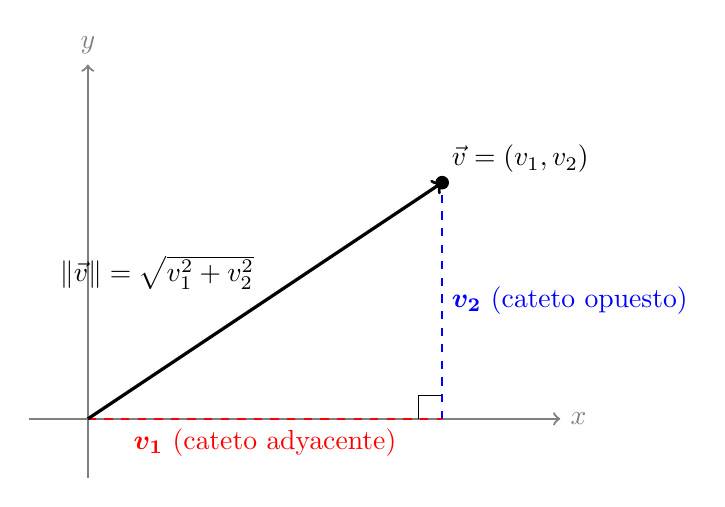
\begin{tikzpicture}[scale=1.5]
    \draw[->, gray, thick] (-0.5,0) -- (4,0) node[right] {$x$};
    \draw[->, gray, thick] (0,-0.5) -- (0,3) node[above] {$y$};

    \draw[dashed, blue, thick] (3,0) -- (3,2);
    \draw[dashed, red, thick] (0,0) -- (3,0);
    
    \draw (2.8,0) -- (2.8,0.2) -- (3,0.2);

    \draw[->, very thick, black] (0,0) -- (3,2) node[midway, above left] {$\|\vec{v}\| = \sqrt{v_1^2 + v_2^2}$};
    
    \node[below, red, font=\boldmath] at (1.5,0) {$v_1$ (cateto adyacente)};
    \node[right, blue, font=\boldmath] at (3,1) {$v_2$ (cateto opuesto)};
    \filldraw[black] (3,2) circle (1.5pt) node[above right] {$\vec{v} = (v_1, v_2)$};
\end{tikzpicture}
\end{center}

\subsubsection{Extensión a $\mathbb{R}^n$}

Este mismo principio geométrico se extiende a dimensiones superiores utilizando la distancia euclidiana. 

\begin{mydefinition}{Norma de un vector en $\mathbb{R}^n$}
Sea $\vec{v} = (v_1, v_2, \dots, v_n)$ un vector en el espacio $\mathbb{R}^n$. La magnitud o norma de $\vec{v}$ se define como la raíz cuadrada de la suma de los cuadrados de sus componentes:
\[ \|\vec{v}\| = \sqrt{v_1^2 + v_2^2 + \dots + v_n^2} \]
\end{mydefinition}

\subsection{Distancia entre dos vectores}

En muchas aplicaciones de ingeniería, es necesario calcular la distancia en línea recta entre dos puntos en el espacio. Si consideramos que estos dos puntos están definidos por los extremos de dos vectores que parten del origen $\vec{u}$ y $\vec{v}$, podemos encontrar esta distancia utilizando las herramientas que ya se definieron: la resta de vectores y la magnitud.

Geométricamente, se sabe que la resta vectorial $\vec{v} - \vec{u}$ produce un nuevo vector que va desde la punta de $\vec{u}$ hasta la punta de $\vec{v}$, representando el desplazamiento exacto entre ambos puntos. 

Por lo tanto, la distancia física entre los extremos de $\vec{u}$ y $\vec{v}$ es simplemente la \textbf{magnitud de su vector diferencia}.

\begin{mydefinition}{Distancia entre vectores en $\mathbb{R}^3$}
Sean $\vec{u} = (u_1, u_2, u_3)$ y $\vec{v} = (v_1, v_2, v_3)$ dos vectores en el espacio tridimensional. La distancia $d$ entre sus puntos finales se define como la norma del vector diferencia $\vec{u} - \vec{v}$:
\[ d(\vec{u}, \vec{v}) = \|\vec{u} - \vec{v}\| \]
    
Dado que la resta de vectores se realiza componente a componente, el vector diferencia es $(u_1 - v_1, u_2 - v_2, u_3 - v_3)$. Al aplicarle la definición de magnitud, se obtiene así por la distancia euclidiana:
\[ d(\vec{u}, \vec{v}) = \sqrt{(u_1 - v_1)^2 + (u_2 - v_2)^2 + (u_3 - v_3)^2} \]

\textit{Nota:} El orden de la resta no importa para el cálculo de la distancia, ya que $\|\vec{u} - \vec{v}\| = \|\vec{v} - \vec{u}\|$. Al elevar al cuadrado las diferencias de las componentes, cualquier signo negativo se vuelve positivo.
\end{mydefinition}

\begin{center}
\shorthandoff{>}
\begin{tikzpicture}[x={(-0.5cm,-0.5cm)}, y={(1cm,0cm)}, z={(0cm,1cm)}, scale=1.5]
    % Ejes
    \draw[->, gray] (0,0,0) -- (3,0,0) node[below left] {$x$};
    \draw[->, gray] (0,0,0) -- (0,4,0) node[right] {$y$};
    \draw[->, gray] (0,0,0) -- (0,0,3) node[above] {$z$};
    
    % Definición de las coordenadas de los vectores
    \coordinate (U) at (2, 1, 2);
    \coordinate (V) at (1, 3, 1);
    
    % Vectores u y v desde el origen
    \draw[->, very thick, blue] (0,0,0) -- (U) node[midway, above left] {$\vec{u}$};
    \draw[->, very thick, red] (0,0,0) -- (V) node[midway, below right] {$\vec{v}$};
    
    % Vector diferencia (representa la distancia)
    \draw[->, very thick, purple] (U) -- (V) node[midway, above right] {$\vec{v} - \vec{u}$};
    
    % Puntos en los extremos para dar énfasis
    \filldraw[black] (U) circle (1.2pt);
    \filldraw[black] (V) circle (1.2pt);
    
    % Cuadro explicativo
    \node[fill=white, draw=black, rounded corners, inner sep=4pt] at (2.5, 3.5, 3) 
    {\footnotesize Distancia $= \|\vec{v} - \vec{u}\|$};
\end{tikzpicture}
\end{center}

\subsection{Vectores unitarios}

En muchas aplicaciones de ingeniería, a menudo se requiere únicamente la dirección y el sentido en el que actúa un fenómeno (como la dirección del flujo de un fluido o la línea de acción de una fuerza), independientemente de su magnitud. Para aislar esta información, se utilizan los vectores unitarios.

\begin{mydefinition}{Vector unitario}
Un vector unitario es aquel cuya magnitud (o longitud) es exactamente igual a 1. Si se denota la magnitud de un vector $\vec{v}$ como $\|\vec{v}\|$, entonces $\vec{v}$ es unitario si:
\[ \|\vec{v}\| = 1 \]
Para distinguirlos del resto, a los vectores unitarios se les suele denotar con un acento circunflejo en lugar de una flecha, por ejemplo, $\hat{u}$.
\end{mydefinition}

\subsubsection{Normalización de un vector}

Cualquier vector $\vec{v}$ que no sea el vector cero puede transformarse en un vector unitario que apunte exactamente en su misma dirección. A este proceso geométrico se le llama \textbf{normalización}. 

Para normalizar un vector, simplemente se multiplica por el recíproco de su propia magnitud:
\[ \hat{u} = \frac{1}{\|\vec{v}\|} \vec{v} = \frac{\vec{v}}{\|\vec{v}\|} \]
De esta manera, el vector resultante $\hat{u}$ conserva la dirección original, pero su tamaño se ha escalado para que sea exactamente 1.

\subsubsection{Vectores unitarios canónicos}

En los sistemas de coordenadas rectangulares, definimos vectores unitarios especiales que apuntan a lo largo de las direcciones positivas de los ejes coordenados. Estos son los vectores base fundamentales, ya que nos permiten expresar cualquier vector en el espacio como una combinación de ellos de forma sencilla (aunque existen múltiples bases para un mismo espacio, estos vectores se les considera canónicos ya que son los más comúnmente utilizados).

En el espacio $\mathbb{R}^3$, estos vectores son:
\begin{itemize}
    \item $\hat{\imath} = (1, 0, 0)$ en la dirección del eje $x$.
    \item $\hat{\jmath} = (0, 1, 0)$ en la dirección del eje $y$;
    \item $\hat{k} = (0, 0, 1)$ en la dirección del eje $z$.
\end{itemize}

Gracias a esto, cualquier vector $\vec{v} = (v_1, v_2, v_3)$ se puede escribir algebraicamente separando sus componentes direccionales:
\[ \vec{v} = v_1\hat{\imath} + v_2\hat{\jmath} + v_3\hat{k} \]

\begin{center}
\shorthandoff{>}
\begin{tikzpicture}[x={(-0.5cm,-0.5cm)}, y={(1cm,0cm)}, z={(0cm,1cm)}, scale=2]
    \draw[->, gray] (0,0,0) -- (2,0,0) node[below left] {$x$};
    \draw[->, gray] (0,0,0) -- (0,2,0) node[right] {$y$};
    \draw[->, gray] (0,0,0) -- (0,0,2) node[above] {$z$};
    
    \draw[->, very thick, red] (0,0,0) -- (1,0,0) node[midway, below right, font=\boldmath] {$\hat{\imath}$};
    \draw[->, very thick, green!60!black] (0,0,0) -- (0,1,0) node[midway, below right, font=\boldmath] {$\hat{\jmath}$};
    \draw[->, very thick, blue] (0,0,0) -- (0,0,1) node[midway, left, font=\boldmath] {$\hat{k}$};
    

    \draw[dashed, gray] (1,0,0) -- (1,-0.2,0) node[below=2pt, black] {\footnotesize 1};
    \draw[dashed, gray] (0,1,0) -- (0,1,-0.2) node[below=2pt, black] {\footnotesize 1};
    \draw[dashed, gray] (0,0,1) -- (-0.2,0,1) node[left=2pt, black] {\footnotesize 1};
\end{tikzpicture}
\end{center}

\subsection{Ejercicios}
Realizar los cálculos en los ejercicios del 1 al 3.

\begin{enumerate}
    \item $ (8a, -2b, 13c) = (52, 12, 11) + \frac{1}{2}(?, ?, ?)$
    \item $ (-21, 23) - (?, 6) = (-25, ?) $
    \item $ (2,3,5) - 4 \hat{\imath} + 3\hat{\jmath} = (?,?,?) $
    \item ¿Qué restricciones se deben de tener sobre $x$, $y$ y $z$ de modo que la terna $(x,y,z)$ represente un punto sobre el eje $y$? ¿Y sobre el eje $z$? ¿En el plano $xz$? ¿En el plano $yz$?
    \item Trazar los vectores $\vec{v} = (2,3,-6)$ y $\vec{w} = (-1,1,1)$. En esa figura trazar $-\vec{v}$, $\vec{v} + \vec{w}$, $2\vec{v}$ y $\vec{v} - \vec{w}$.
    \item Dos personas jalan horizontalmente de cuerdas atadas a un poste; el ángulo entre las cuerdas es de $60^\circ$. A jala con una fuerza de $150$ lb y B jala con una fuerza de $100$ lb.
\begin{enumerate}
    \item La fuerza resultante es la suma vectorial de las dos fuerzas en un sistema coordenado escogido de manera conveniente. Trazar una figura a escala que represente graficamente a las tres fuerzas.
    \item Usando trigonometría, determinar fórmulas para las componentes vectoriales de las dos fuerzas en un sistema coordenado escogido de manera conveniente. Efectuar la suma algebraica y hallar el ángulo que la fuerza resultante forma con la cuerda de A.
\end{enumerate}
    \item La velocidad $\vec{v_1}$ del viento es de $ 40 \frac{mi}{h} $ de este a oeste, mientras que un aeroplano viaja con velocidad en el aire $ \vec{v_2} = 100 \frac{mi}{h} $ hacia el norte. La rapidez del aeroplano respecto a la tierra es la magnitud de la suma vectorial $\vec{v_1} + \vec{v_2}$.
\begin{enumerate}
    \item Hallar $\vec{v_1} + \vec{v_2}$.
    \item Trazar una figura a escala.
\end{enumerate}
    \item Dado el vector $\vec{v} = (3, -4)$, calcular su magnitud $\|\vec{v}\|$ y encontrar el vector unitario $\hat{u}$ que apunta en la misma dirección que $\vec{v}$. Verificar que $\|\hat{u}\| = 1$.
    \item Calcular la distancia entre los puntos $P = (1, -2, 4)$ y $Q = (3, 1, -1)$ en $\mathbb{R}^3$. Expresar el vector $\overrightarrow{PQ}$ en términos de los vectores unitarios canónicos $\hat{\imath}$, $\hat{\jmath}$ y $\hat{k}$.
    \item Sean $\vec{u} = (2, -1, 3)$ y $\vec{v} = (-1, 4, 2)$. Calcular cada una de las siguientes expresiones:
\begin{enumerate}
    \item $3\vec{u} - 2\vec{v}$
    \item $\|\vec{u} + \vec{v}\|$
    \item $\|\vec{u}\| - \|\vec{v}\|$
\end{enumerate}
¿Por qué en general $\|\vec{u} + \vec{v}\| \neq \|\vec{u}\| + \|\vec{v}\|$?
    \item Un dron parte del punto $A = (0, 0, 0)$ y se desplaza al punto $B = (3, 4, 0)$, luego sube verticalmente hasta el punto $C = (3, 4, 5)$.
\begin{enumerate}
    \item Hallar los vectores de desplazamiento $\overrightarrow{AB}$ y $\overrightarrow{BC}$.
    \item Determinar el desplazamiento total $\overrightarrow{AC}$ como suma vectorial.
    \item Calcular la distancia total recorrida y la distancia en línea recta entre $A$ y $C$. ¿Son iguales? ¿Por qué?
\end{enumerate}
    \item Encontrar todos los valores del escalar $t \in \mathbb{R}$ para los cuales el vector $\vec{w} = (t, 2t-1, 3)$ tenga magnitud igual a $\sqrt{14}$.
    \item Demostrar algebraicamente, usando la definición componente a componente, las siguientes propiedades del álgebra vectorial para vectores en $\mathbb{R}^n$:
\begin{enumerate}
    \item $\kappa(\vec{u} + \vec{v}) = \kappa\vec{u} + \kappa\vec{v}$ \quad (distributividad del escalar sobre la suma vectorial)
    \item $(\kappa + \lambda)\vec{u} = \kappa\vec{u} + \lambda\vec{u}$ \quad (distributividad del escalar sobre la suma escalar)
\end{enumerate}
\end{enumerate}